\documentclass[nobib]{tufte-handout}

\title{Föreläsning 7: Dyck-stigar och Catalantal $\cdot$ 1MA020}

\author[Vilhelm Agdur]{Vilhelm Agdur\thanks{\href{mailto:vilhelm.agdur@math.uu.se}{\nolinkurl{vilhelm.agdur@math.uu.se}}}}

\date{14 februari 2023}


%\geometry{showframe} % display margins for debugging page layout

\usepackage{graphicx} % allow embedded images
  \setkeys{Gin}{width=\linewidth,totalheight=\textheight,keepaspectratio}
  \graphicspath{{graphics/}} % set of paths to search for images
\usepackage{amsmath}  % extended mathematics
\usepackage{booktabs} % book-quality tables
\usepackage{units}    % non-stacked fractions and better unit spacing
\usepackage{multicol} % multiple column layout facilities
\usepackage{lipsum}   % filler text
\usepackage{fancyvrb} % extended verbatim environments
  \fvset{fontsize=\normalsize}% default font size for fancy-verbatim environments

\usepackage{graphicx}
\usepackage{subfig}

\usepackage{color,soul} % Highlights for text


\include{mathcommands.extratex}

\begin{document}

\definecolor{darkgreen}{rgb}{0.0627, 0.4588, 0.1451}

\maketitle% this prints the handout title, author, and date

\begin{abstract}
\noindent
Vi introducerar Dyck-stigar, och härleder en rekursion för deras antal. Sedan använder vi rekursionen för att hitta en genererande funktion, och använder genererande funktionen för att ge en explicit formel för deras antal.

Efter det ger vi ett kombinatoriskt bevis för vår formel för antalet Dyck-stigar, som är betydligt kortare.

Slutligen ger vi två till exempel på saker som räknas av Catalantalen.
\end{abstract}

\section{Dyck-stigar}

\begin{definition}
    En \emph{gitterstig} på $\Z^2$ av längd $n$ mellan $a$ och $b$ börjar i punkten $a$ och tar sig sedan till punkten $b$ med $n$ stycken steg, som kan vara upp, ner, höger, eller vänster.\sidenote[][-0.3cm]{Vi kan betrakta en sådan stig som ett ord av längd $n$ ur alfabetet $\{U,N,H,V\}$, tillsammans med en startpunkt.}
    \begin{figure}
        \centering
        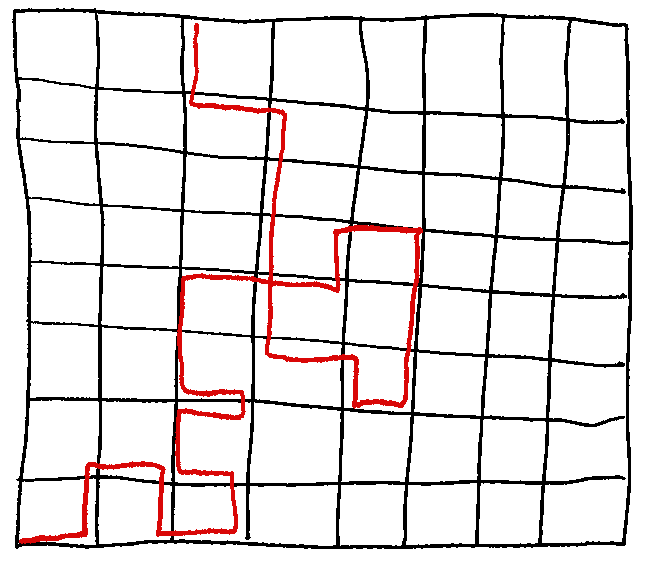
\includegraphics[width=0.5\textwidth]{graphics/general_lattice_path.png}
        \caption{En gitterstig av längd $28$ från $(0,0)$ till $(2,8)$.}
    \end{figure} 
\end{definition}

Det finns uppenbarligen $4^n$ gitterstigar av längd $n$ med en given startpunkt, om vi inte kräver att den skall sluta i någon given punkt.

\begin{definition}
    En \emph{uppåt-höger-stig} på $\Z^2$ från $a$ till $b$ är en gitterstig mellan $a$ och $b$ som enbart tar steg uppåt och åt höger.\sidenote[][]{I tolkningen av stigar som ord är alltså dessa ord ur det mindre alfabetet $\{U,H\}$.}
    \begin{figure}[h]
        \centering
        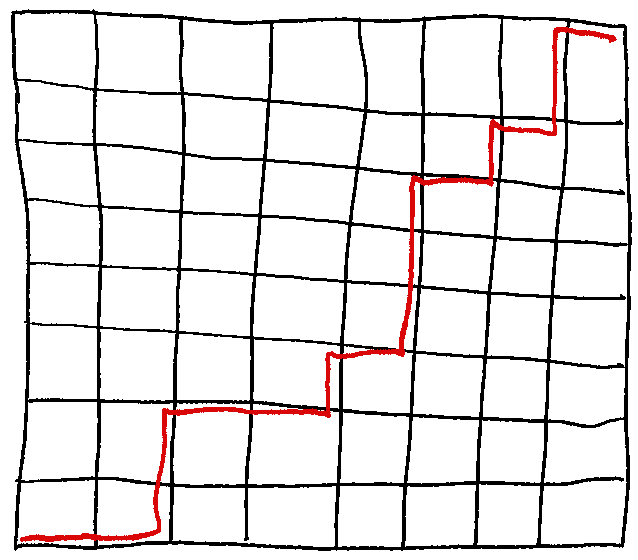
\includegraphics[width=0.5\textwidth]{graphics/right_up_lattice_path.png}
        \caption{En uppåt-höger-stig från $(0,0)$ till $(8,8)$ av längd sexton.}
    \end{figure}
\end{definition}

Notera att till skillnad från allmänna gitterstigar bestäms en uppåt-höger-stigs längd av dess start och slutpunkt, eftersom den inte kan ta några omvägar eller gå baklänges. En stig från $(0,0)$ till $(a,b)$ kommer alltid att ta precis $a$ steg uppåt och $b$ steg till höger, det enda som kan variera är i vilken ording stegen tas.

Alltså ges det totala antalet uppåt-höger-stigar från $(0,0)$ till $(a,b)$ av $\binom{a+b}{a}$, eftersom det är antalet sätt att välja de $a$ ställen vi tar ett steg höger av totalt $a+b$ steg.

\begin{definition}
    En Dyck-stig av längd $2n$ är en uppåt-höger-stig från $(0,0)$ till $(n,n)$ som aldrig går under diagonalen.
    \begin{figure}
        \centering
        \includegraphics*[width=0.5\textwidth]{graphics/Dyck_path.png}
        \caption{En Dyck-stig av längd sexton.}
    \end{figure}
\end{definition}

Notera att en Dyck-stig alltid måste börja med ett steg uppåt och sluta med ett steg åt höger, eftersom den annars ju hade varit under diagonalen.

Hur många Dyck-stigar finns det av varje given längd? Vi kan använda vår observation om att de alltid börjar med ett upp-steg för att ge en rekursion för detta antal:

\begin{lemma}\label{dyck_path_recursion_lemma}
    Låt $d_n$ beteckna antalet Dyck-stigar av längd $2n$. Då gäller det för alla $n \geq 0$ att
    $$d_{n+1} = \sum_{k=0}^{n} d_k d_{n-k}$$
    och $d_0 = 1$.\sidenote[][]{Antalet ord av längd noll anser vi vara ett, eftersom det bara finns ett sätt att välja ett sådant.}

    \begin{proof}
        Överväg en Dyck-stig av längd $2(n+1)$. Vi kan dela upp den i två kortare Dyck-stigar som följer: Den börjar med ett upp-steg, som vi färgar grått. Sedan fortsätter den i ett tag tills den träffar diagonalen för första gången. Vi färgar alla steg innan det steg i vilken den träffar diagonalen blåa, och steget i vilken den träffar diagonalen grått. Sedan färgar vi resten av stegen röda.

        \begin{figure}
            \centering
            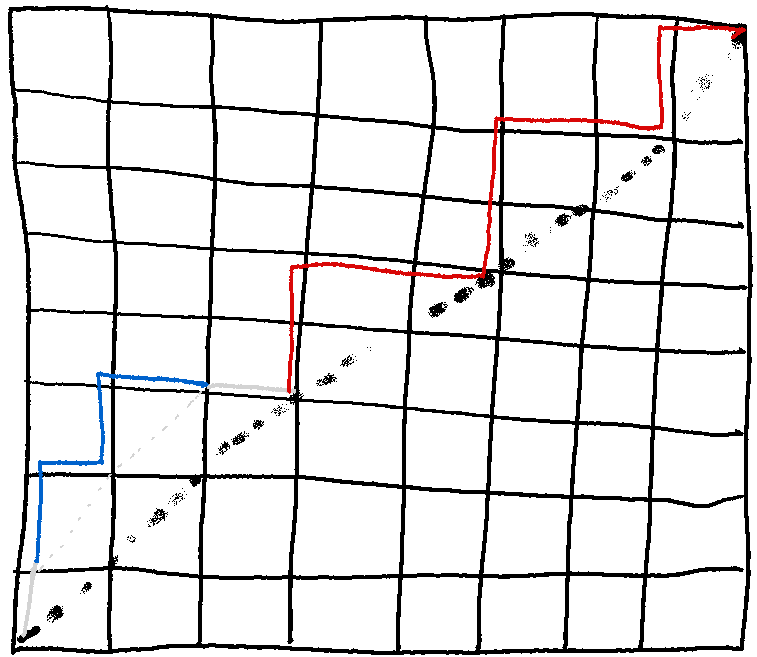
\includegraphics[width = 0.6\textwidth]{graphics/Dyck_path_recursion.png}
            \caption{En illustration av vår uppdelning av en\, Dyck-stig i gråa, blåa, och röda steg.}
        \end{figure}

        Vi hävdar att de blå stegen utgör en Dyck-stig av längd $2k$ för något $0 \leq k \leq n$, och de röda stegen utgör en Dyck-stig av längd $2(n-k)$, så att vi tillsammans med de två gråa stegen har totalt $2k + 2(n-k) + 2 = 2(n+1)$ steg. Ekvivalent, i tolkningen av stigar som ord, så säger vi att ordet för stigen vi började med kan skrivas som
        $$Uw_1Hw_2$$
        för två kortare\sidenote[][]{Det är tillåtet att de är av längd noll.} Dyck-stigar $w_1$ och $w_2$.

        Vi kan välja $k$ fritt mellan $0$ och $n$, och vi kan sedan välja våra två kortare Dyck-stigar helt fritt så länge de har rätt längd, så multiplikations- och additionsprincipen ger oss att vi kan totalt välja på
        $$\sum_{k=0}^{n} d_k d_{n-k}$$
        sätt, vilket är vad vi ville bevisa.
    \end{proof}
\end{lemma}

Den uppmärksamme bland er kanske redan känt igen att den här rekursionen säger något om en faltning -- specifikt säger den att
$$d_{n+1} = (d * d)_n,$$
vilket ser ut som något vi borde kunna använda för att räkna ut genererande funktionen av den här följden.

\begin{proposition}
    Den genererande funktionen för $\{d_k\}_{k=0}^\infty$, antalet Dyck-stigar, är
    $$F_d(x) = \frac{1 - \sqrt{1 - 4x}}{2x}.$$

    \begin{proof}
        Vi observerar att Lemma \ref{dyck_path_recursion_lemma} ger oss att för alla $n \geq 0$ så är
        $$d_{n+1} = (d*d)_n,$$
        så om vi tar genererande funktioner av bägge sidorna ser vi att vänster led blir
        $$\sum_{n=0}^{\infty}d_{n+1}x^n = \frac{1}{x}\sum_{n=0}^{\infty} d_{n+1} x^{n+1} = \frac{F_d(x) - 1}{x}$$
        och höger led blir
        $$F_{d * d}(x) = F_d(x)^2$$
        så att vi har att
        $$F_d(x) = x F_d(x)^2 + 1.$$

        Det här är ju bara en vanlig andragradsekvation som vi kan lösa för $F_d$, och få att
        $$F_d(x) = \frac{1 \pm \sqrt{1 - 4x}}{2x}.$$

        Det enda som återstår är att se om den rätta lösningen har ett plus- eller minustecken. Sättet vi ser detta på är att vi vet vad den skall ta för värde i en specifik punkt -- vi kan ju nämligen räkna att
        $$F_d(0) = \sum_{k=0}^{\infty} d_k 0^k = d_0 = 1$$
        så funktionen måste vara ett i noll.

        En snabb räkning ger oss att
        $$\lim_{x \to 0} \frac{1 - \sqrt{1 - 4x}}{2x} = 1$$
        emedan gränsvärdet
        $$\lim_{x \to 0} \frac{1 + \sqrt{1 - 4x}}{2x}$$
        inte existerar. Alltså måste den korrekta lösningen vara med minustecknet, såsom önskat.
    \end{proof}
\end{proposition}

Så, hittills har vi definierat våra Dyck-stigar, listat ut en rekursion för deras antal, och använt denna rekursion för att härleda en genererande funktion. Kan vi använda denna genererande funktion för att härleda en explicit formel för antalet Dyck-stigar?

Svaret på den frågan är ja, men det kräver ett lemma vi inte sett ännu.

\section{Newtons binomialsats, och en explicit formel för $d_n$}

\begin{definition}
    För varje $x\in \R$ och varje $k \in \Z^{\geq 0}$ ges den \emph{fallande fakulteten} $x^{\underline{k}}$ av\sidenote[][]{Så produkten har $k$ termer. I fallet med $k=0$ får vi en tom produkt, vilket vi konventionellt anser är ett, så $x^{\underline{0}} = x^{\overline{0}} = 1$ för alla $x$.}
    $$x^{\underline{k}} = x(x-1)(x-2)\ldots(x-(k-1))$$
    och den \emph{stigande fakulteten} $x^{\overline{k}}$ av
    $$x^{\overline{k}} = x(x+1)(x+2)\ldots(x+k-1).$$

    Om $x$ är ett heltal ges alltså $x^{\underline{k}}$ av $\frac{x!}{k!}$ och $x^{\overline{k}}$ av $\frac{(x+k-1)!}{(x-1)!}$.
\end{definition}

Vi kan särskilt notera att när $x$ är ett heltal ges antalet permutationer av längd $k$ ur ett alfabete med $x$ bokstäver alltså av $x^{\underline{k}}$, och således har vi också att
$$\binom{x}{k} = \frac{x^{\underline{k}}}{k!}$$
för alla heltal $x$ och $k$. Men detta uttrycket är ju helt väldefinierat även om $x$ inte är ett heltal, vilket motiverar oss att göra följande definition:

\begin{definition}
    För alla $x \in \R$ och $k \in \Z^{\geq 0}$ säger vi att
    $$\binom{x}{k} = \frac{x^{\underline{k}}}{k!}.$$
\end{definition}

Anledningen att vi gör allt detta arbetet är att det låter oss generalisera binomialsatsen även till potenser som inte är heltal, såsom Newton upptäckte.

\begin{theorem}[Newtons binomialsats]
    För alla $x$ och $y$ och $r \in \R$ gäller det att
    $$(x + y)^r = \sum_{k=0}^{\infty} \binom{r}{k} x^{r-k} y^k$$

    \begin{proof}
        Taylorutveckla.\sidenote[][]{Ett bevis återfinns lätt med google, men eftersom det inte egentligen har något med kombinatorik att göra utelämnar vi det i denna kursen.}
    \end{proof}
\end{theorem}

Låt oss nu tillämpa vår nya kunskap på Dyckstigarna. Eftersom den genererande funktionen vi fann för deras antal involverade en kvadratrot kommer vi ju vilja tillämpa Newtons binomialsats i fallet med $r = \frac{1}{2}$, så låt oss börja med ett lemma om vad som händer i just det fallet.

\begin{theorem}\label{theorem_dyck_paths_counted_by_catalan}
    Antalet Dyck-stigar $d_n$ ges av
    $$d_n = \frac{1}{n + 1}\binom{2n}{n}.$$

    I själva verket är dessa tal så viktiga att de har sitt egna namn -- de kallas för \emph{Catalan-talen}.

    \begin{proof}
        Vi vet att den genererande funktionen för denna följd ges av
        $$F_d(x) = \sum_{k=0}^{\infty} d_k x^k = \frac{1 - \sqrt{1 - 4x}}{2x}$$
        så vi behöver serieutveckla detta uttryck.

        Newtons binomialsats säger oss att
        $$\sqrt{1 + y} = \sum_{k=0}^{\infty} \binom{1/2}{k} y^k$$
        så om vi sätter in $y = -4x$ får vi att
        $$\sqrt{1 - 4x} = \sum_{k=0}^{\infty} (-1)^k \binom{1/2}{k} 4^k x^k.$$
        
        När $k=0$ så blir $\binom{1/2}{0} = \frac{(1/2)^{\underline{0}}}{0!} = \frac{1}{1}$, och alltså är hela nollte termen lika med ett. Så alltså gäller det att
        \begin{align*}
            \frac{1 - \sqrt{1 - 4x}}{2x} &= \frac{\sum_{k=1}^{\infty} (-1)^{k-1} \binom{1/2}{k} 4^k x^k}{2x}\\
            &= \sum_{k=1}^{\infty} 2(-1)^{k-1} \binom{1/2}{k} 4^{k-1} x^{k-1}\\
            &= \sum_{k=0}^{\infty} 2 (-4)^{k}\binom{1/2}{k+1} x^k
        \end{align*}
        från vilket vi kan läsa av att
        $$d_n = 2 (-4)^{n}\binom{1/2}{n+1}.$$

        Låt oss nu försöka förenkla denna formel. Vi börjar med att skriva ut vad definitionen av $\binom{1/2}{n+1}$ är, och får att
        \begin{align*}
            d_n &= 2 (-4)^{n}\binom{1/2}{n+1}\\
            &= 2 (-4)^n \frac{(1/2)^{\underline{n+1}}}{(n+1)!}\\
            &= 2 (-4)^n \frac{(1/2)(1/2 - 1)(1/2 - 2)\ldots(1/2 - n)}{(n+1)!}\\
            &= 2 (-4)^n \frac{(1/2)(-1/2)(-3/2)(-5/2)\ldots(-(2n-1)/2)}{(n+1)!}\\
            &= (-4)^n \frac{(-1)^n 1\cdot3\cdot5\cdot\ldots\cdot(2n-1)}{2^n (n+1)!}\\
            &= 2^n \frac{1}{(n+1)!}\left(\prod_{k \in [2n], k \not\in2\Z} k\right).
        \end{align*}

        Nu kan vi observera att
        $$\prod_{k \in [2n], k \not\in2\Z} k = \left(\prod_{k \in [2n], k \not\in2\Z} k\right)\frac{\prod_{k \in [2n], k \in2\Z} k}{\prod_{k \in [2n], k \in2\Z} k} = \frac{(2n)!}{\prod_{k \in [2n], k \in2\Z} k}$$
        och om vi bryter ut en tvåa ur varje term i produkten över alla jämna heltal ser vi att
        $$\prod_{k \in [2n], k \in2\Z} k = 2^n n!$$
        så sammantaget har vi sett att
        $$\prod_{k \in [2n], k \not\in2\Z} k = \frac{(2n)!}{2^n n!}.$$

        Om vi stoppar in detta i vårt uttryck för $d_n$ vi hade innan så ser vi att
        \begin{align*}
            d_n &= 2^n \frac{1}{(n+1)!}\left(\prod_{k \in [2n], k \not\in2\Z} k\right)\\
            &= 2^n \frac{1}{(n+1)!}\frac{(2n)!}{2^n n!}\\
            &= \frac{(2n)!}{(n+1)!(n!)} = \frac{1}{n+1} \frac{(2n)!}{n!n!} = \frac{1}{n+1}\binom{2n}{n},
        \end{align*}
        vilket är formeln vi ville bevisa.
    \end{proof}
\end{theorem}

Så vi har till slut hittat en fin formel för antalet Dyck-stigar, och alltså för Catalantalen. Tyvärr var vägen vi tog dit väldigt lerig, i botten på en hopväxt och snårig dal. Finns det ett mindre kladdigt sätt att hitta denna formel?\sidenote[][]{Vårt arbete med att ta fram denna formel för antalet Dyck-stigar illustrerar både för- och nackdelarna med metoden med genererande funktioner. Det är en pålitlig metod, med tydliga steg för vad vi vill göra -- efter att vi hittade rekursionen vi började med behövde vi aldrig egentligen vara kreativa, utan vi kom fram till målet genom att bara följa vårt recept.

Å andra sidan kan räkningarna man behöver göra för att tillämpa metoden vara väldigt fula. Vad man köper i standardisering får man betala för i begriplighet -- det är nog svårt att säga att man begriper \emph{varför} den formeln ger Catalantalen efter att ha sett vårt bevis.}

\section{Ett kombinatoriskt bevis för formeln för Catalantalen}

\begin{proof}[Ett kombinatoriskt bevis av Teorem \ref{theorem_dyck_paths_counted_by_catalan}]
    Låt oss överväga samlingen av alla uppåt-höger-stigar från $(0,0)$ till $(n,n)$. Vi kallar varje stig som passerar under diagonalen för en \emph{dålig} stig -- mängden av sådana är uppenbarligen komplementet till mängden av Dyck-stigar. Så om vi kan räkna de dåliga stigarna får vi också antalet Dyck-stigar, eftersom vi vet att det totala antalet uppåt-höger-stigar från $(0,0)$ till $(n,n)$ är precis $\binom{2n}{n}$.

    Sättet vi räknar antalet dåliga stigar är att påvisa en bijektion mellan dem och mängden av uppåt-höger-stigar från $(0,0)$ till $(n+1,n-1)$.

    \begin{figure}\label{fig:dyck_comb_proof_path}
        \centering
        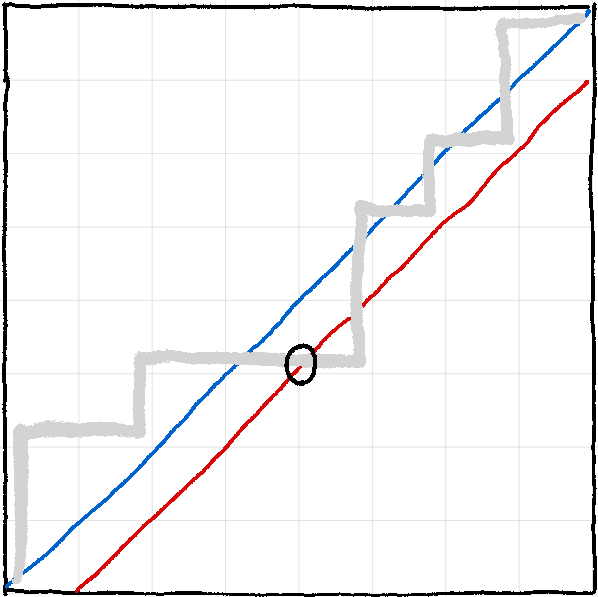
\includegraphics[width=0.6\textwidth]{graphics/dyck_combinatorial_proof_path.png}
        \caption{En av våra dåliga stigar, med huvuddiagonalen i blått och första diagonalen under huvuddiagonalen i rött. Punkten där stigen träffar den första underdiagonalen markeras med en cirkel.}
    \end{figure}

    Givet en dålig stig markerar vi första punkten på vilken den träffar första underdiagonalen, alltså diagonalen under huvuddiagonalen. Att det måste finnas en sådan punkt följer av att stigen är dålig -- om den aldrig träffade den underdiagonalen vore stigen en Dyckstig.

    Sedan speglar vi resten av stigen, efter punkten vi markerade, i första underdiagonalen. Vi ersätter alltså varje steg uppåt med ett steg till höger, och varje steg till höger med ett steg uppåt. 

    \begin{figure}\label{fig:dyck_comb_proof_reflected_path}
        \centering
        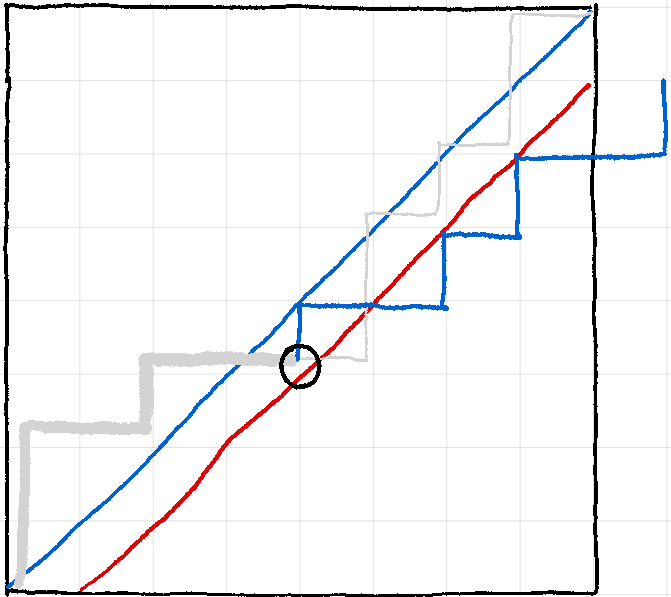
\includegraphics[width = 0.6\textwidth]{graphics/dyck_combinatorial_proof_reflected_path.png}
        \caption{Den uppåt-höger-stig från $(0,0)$ till $(n+1,n-1)$ som motsvarar vår dåliga stig i förra figuren. Stigen är grå fram tills punkten där vi började spegla den, och fortsätter sedan i blått. Originalstigen fortsätter i grått.}
    \end{figure}

    Eftersom vi i punkten vi började spegla just träffat första underdiagonalen så måste vi i den punkten ha haft ett steg mer åt höger än uppåt. Totalt har vi, i originalstigen, lika många steg uppåt som åt höger, så återstoden av den efter den punkten måste ha ett steg mer uppåt än åt höger.

    När vi speglar blir varje steg uppåt ett åt höger, och vice versa, så vår speglade stig måste ha ett steg mer åt höger än uppåt också i biten efter speglingen. Alltså måste den resulterande stigen efter speglingen ha två steg fler åt höger än uppåt, och alltså hamna i $(n+1,n-1)$.\sidenote[][-1cm]{I symboler har vi $u_i$ steg \emph{u}ppåt i stigen \emph{i}nnan punkten vi speglar efter, och $h_i$ steg åt \emph{h}öger. Efter punkten vi speglar \emph{e}fter har vi $u_e$ steg uppåt och $h_e$ steg åt höger. Så i Figur \ref{fig:dyck_comb_proof_path} så har vi $u_i = 3$, $h_i = 4$, $u_e = 5$, och $h_e = 4$.
    
    Så för stigen vi börjar med har vi $h_i = u_i + 1$, och $h_i + h_e = n$ samt $u_i + u_e = n$ för att den skall sluta i $(n,n)$. Stigen efter speglingen kommer att ha $h_i + u_e$ steg åt höger och $u_i + h_e$ steg uppåt. Om man arbetar sig igenom dessa ekvationer kommer man att se att vi verkligen har $n+1$ steg åt höger och $n-1$ steg uppåt i den reflekterade stigen.}

    Så vi har hittat ett sätt att skicka en dålig stig på en stig från $(0,0)$ till $(n+1,n-1)$. För att detta skall vara en bijektion måste processen vara reversibel - givet en stig från $(0,0)$ till $(n+1,n-1)$ måste vi kunna återskapa den motsvarande dåliga stigen.

    Sättet vi gör det på är samma som innan -- vi hittar första punkten i vilken vår stig träffar första underdiagonalen, och speglar efter den. Att en sådan punkt måste finnas är uppenbart, eftersom $(0,0)$ ligger ovanför den underdiagonalen, och $(n+1,n-1)$ ligger under den. Så för att ta oss från ena sidan av den till andra måste vi passera den.

    Att denna spegling kommer ge oss rätt dåliga stig är enkelt att se -- allt vi gjort är att spegla två gånger, vilket så klart inte gör någonting.

    Alltså har vi bevisat att antalet dåliga stigar är lika med antalet stigar från $(0,0)$ till $(n+1,n-1)$. Vi vet att det finns $\binom{(n + 1) + (n - 1)}{n+1}$ sådana stigar, så vi kan räkna att
    \begin{align*}
        d_n &= \abs{\text{stigar }(0,0)\to(n,n)} - \abs{\text{dåliga stigar}}\\
        &= \binom{2n}{n} - \binom{2n}{n+1}\\
        &= \frac{(2n)!}{n!n!} - \frac{(2n)!}{(n+1)!(n-1)!}\\
        &= (2n)!\left(\frac{(n+1)}{(n+1)!n!} - \frac{n}{(n+1)!n!}\right)\\
        &= \frac{(2n)!}{(n+1)!n!} = \frac{1}{n+1}\frac{(2n)!}{n!n!} = \frac{1}{n+1}\binom{2n}{n}
    \end{align*}
    vilket bevisar satsen.
\end{proof}

Så vårt kombinatoriska bevis undvek helt att behöva fundera på rekursioner och genererande funktioner. Det är en mycket mer direkt rutt till vårt mål, men vi missade några sevärdheter längs vägen.\sidenote[][]{Hur man hade härlett vår rekursion eller den genererande funktionen givet bara vad vi lärde oss i det kombinatoriska beviset är långt ifrån uppenbart.}

\section{Fler saker som räknas av Catalantalen}

Som vi nämnde tidigare är Catalantalen viktiga eftersom de räknar fler saker än bara just Dyck-stigar. I nästa föreläsning kommer vi se ett viktigt exempel. Nu, i slutet på denna, tar vi några mindre exempel.

\begin{example}
    Antalet sätt att skriva $2n$ matchande parenteser räknas av Catalantalen. Med matchande parenteser menar vi alltså ett uttryck som $(()(()))()(())$ -- och i ett uttryck som $)((()$ matchar de inte. Varje $($ måste ha en motsvarande $)$ senare i ordet, och varje $)$ måste ha ett matchande $($ tidigare i ordet.

    Hur bevisar vi att detta räknas av Catalantalen? Jo, vi ser att detta lyder samma rekursion som Dyck-stigarna gjorde. Varje uttryck med matchande parenteser måste börja med $($, och denna första startparentes måste matcha en slutparentes. Det som står inom dessa parenteser måste också vara ett matchande uttryck, och likaså det som står efter slutparentesen som matchar första parentesen.

    Alltså kan vi skriva varje uttryck med matchande parenteser på formen $(w_1)w_2$, med $w_1$ och $w_2$ två kortare matchande uttryck. Det här är precis samma uppdelning som vi hade för våra Dyckstigar, så det kommer ge samma rekursion, och alltså är det samma följd.\sidenote[][-2cm]{Vi hade också, vilket kanske vore enklare, helt enkelt kunnat se att det finns en bijektion mellan matchande uttryck med parenteser och Dyck-stigar, genom att tolka $($ som ``steg uppåt'' och $)$ som ``steg till höger''.}
\end{example}

\begin{example}\label{example_polygons}
    Det problem som ursprungligen fick upp matematikers intresse i väst\sidenote[][-0.6cm]{De studerades först av en matematiker i Kina på 1700-talet vid namn Minggatu, som använde dem för att ge identiteter för sinus-funktionen, i stil med
    $$\sin(2\alpha) = 2\sin(\alpha) - \sum_{n=1}^{\infty} \frac{C_{n-1}}{4^{n-1}}\sin^{2n+1}(\alpha).$$} för Catalantalen var att dela upp en konvex polygon med $n+2$ sidor i trianglar, genom att rita streck mellan hörnen som inte korsar varandra.

    \begin{figure}
        \centering
        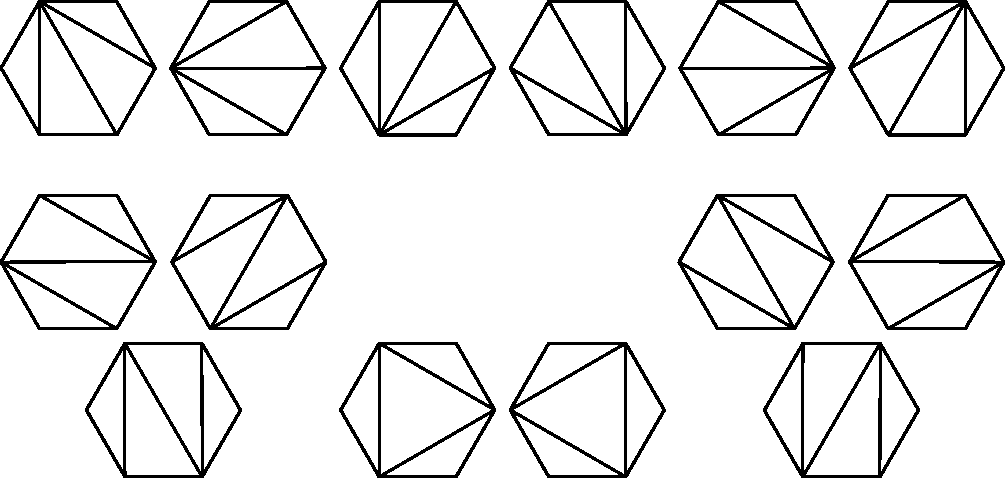
\includegraphics[width = 0.5\textwidth]{graphics/Catalan-Hexagons-example.pdf}
        \caption{Fallet med hexagoner.}
    \end{figure}

    Det här problemet studerades först av Euler\sidenote[][]{Som ju redan har mer än tillräckligt med saker namngivna efter sig, så det är tur att vi inte döpte talen efter honom.}, och beviset att de räknas av Catalantalen utvecklades av Segner, Goldbach, och Lamé. Vår rekursion för Catalantalen brukar kallas för Segnerrekursionen.

    Senare studerades problemet med parentetiseringar av Eugène Charles Catalan, efter vilken talen fick sitt namn på femtiotalet.
\end{example}

\section{Övningar}

\begin{xca}
    Hur många gitterstigar av längd $n$ från $(0,0)$ till $(a,b)$ finns det?
\end{xca}

\begin{xca}
    Bevisa att antalet uppdelningar av en konvex polygon med $n+2$ sidor i trianglar, såsom vi diskuterade i Exempel \ref{example_polygons}, räknas av Catalantalen.\sidenote[][]{Ledtråd: Tänk kombinatoriskt, och se att dessa också lyder vår rekursion.}
\end{xca}

\begin{xca}
    Betrakta mängden av följder av heltal av längd $n$, som
    \begin{itemize}
        \item börjar med $1$,
        \item och om det föregående talet är $k$ är nästa tal vilket tal som helst mellan $1$ och $k+1$.
    \end{itemize} 

    För $n = 4$ är dessa följder
    $$1234, 1233, 1232, 1231, 1223, 1222, 1221, 1212, 1211, 1123, 1122, 1121, 1112, 1111.$$

    Bevisa att antalet av dessa följder ges av Catalantalen.
\end{xca}

\begin{xca}
    Bevisa att alla följderna på denna lista är lika med Catalantalen:
    \begin{enumerate}
        \item Antalet ord ur alfabetet $\{-1, 1\}$ med $n$ stycken av varje bokstav, sådana att alla partialsummor är ickenegativa. Det vill säga, om vi tar summan av de första $k$ bokstäverna i ordet skall det inte bli negativt, för alla $0 \leq k \leq 2n$.
        \item Följder $1 \leq a_1 \leq a_2 \leq \ldots \leq a_n$ av heltal, med $a_i \leq i$ för alla $i$.
        \item En valfri följd från Richard Stanleys lista av 66 saker som räknas av Catalantalen\sidenote[][]{Denna lista återfinns här: \url{https://math.mit.edu/~rstan/ec/catalan.pdf}}, som inte redan dykt upp i föreläsningen eller i en annan övning.
    \end{enumerate}
\end{xca}

\begin{xca}
    Vi skriver talen $1$ till $n$ i ordning runt en cirkel.\sidenote[][]{Visst är ni glada att jag inte valde att formulera detta som ``$n$ personer runt ett runt bord?''?} Vi säger att en mängdpartition $\{A_1, A_2, \ldots, A_k\}$ av $[n]$ är \emph{ickekorsande} ifall det, när vi ritar streck mellan alla tal som ligger i samma del av partitionen, aldrig händer att två streck som hör till olika delar korsar varandra. Alltså, närhelst $a, b \in A_i$ och $c, d \in A_j$ så korsar inte strecket $ab$ strecket $cd$. Se figur \ref{fig:two_noncrossing_partitions} för två exempel på ickekorsande partitioner då $n=9$, och figur \ref{fig:crossing_partition} för ett exempel på en korsande partition.
    
    \begin{figure}
        \centering
        \subfloat[\centering $\{\{1,8,9\}, \{2,5,6,7\}, \{3,4\}\}$.]{{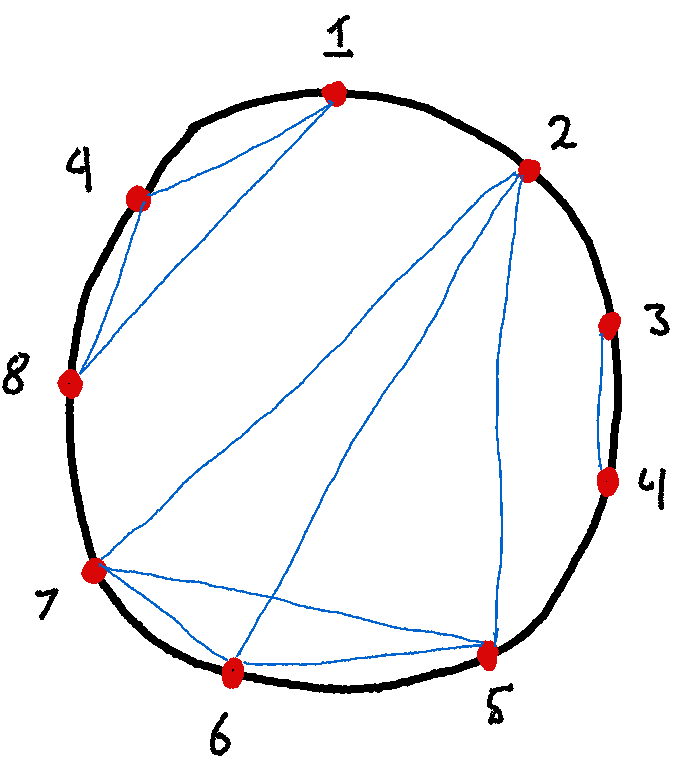
\includegraphics[width=.35\linewidth]{graphics/noncrossing_partition.png}}}\quad
        \subfloat[\centering $\{\{1,3,4\},\{2\},\{5,6,9\},\{7,8\}\}$.]{{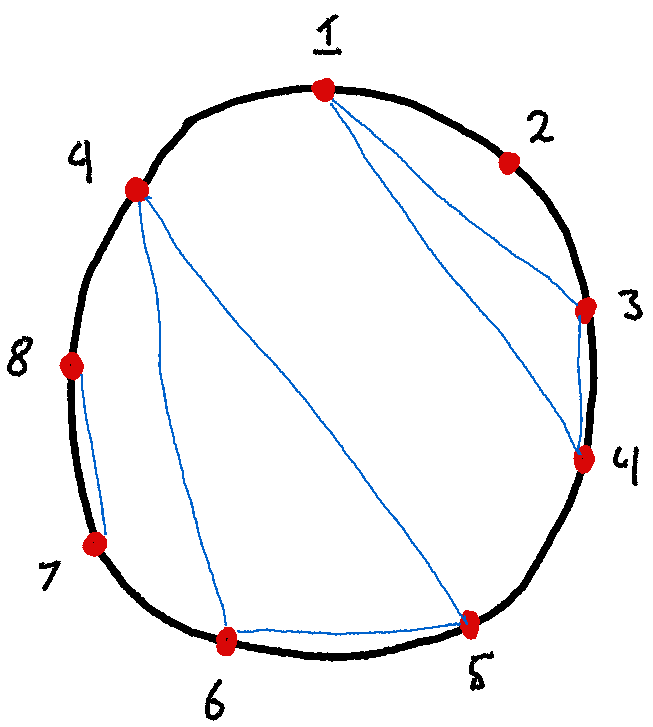
\includegraphics[width=.35\linewidth]{graphics/noncrossing_partition_two.png}}}
        
        \caption{Två stycken ickekorsande mängdpartitioner.}
        \label{fig:two_noncrossing_partitions}
    \end{figure}

    \begin{figure}
        \centering
        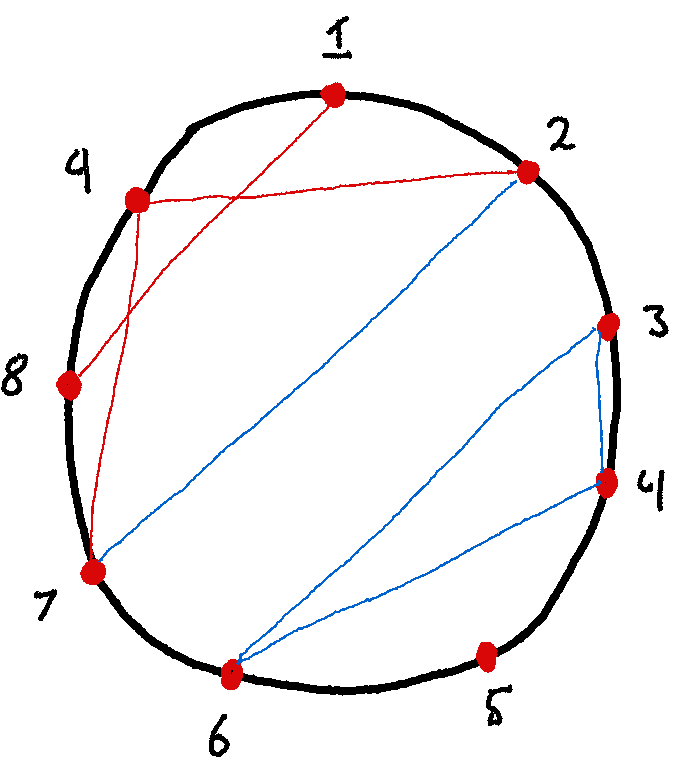
\includegraphics[width=0.5\textwidth]{graphics/crossing_partition.png}
        \caption{Den korsande partitionen $\{\{1,8\},\{2,7,9\},\{3,4,6\},\{5\}\}$, med de korsande strecken\, i rött.}
        \label{fig:crossing_partition}
    \end{figure}

    Bevisa att antalet ickekorsande partitioner räknas av Catalantalen.\sidenote[][]{Ledtråd: Fundera på strecket mellan $9$ och $5$ i den högra av våra två exempel på ickekorsande partitioner. Kan ni se en rekursion?}
\end{xca}

\newpage

%\bibliography{references}
%\bibliographystyle{plainnat}

\end{document}
